\section{Codebook, queries and reporting checklist}
\label{app:codebook}

\subsection{Evidence codebook}
Each study--requirement pair is coded once, by the study's primary finding for that requirement, for \emph{detector} use as defined in \cref{sec:intro}; judge use is never coded.
\begin{description}[leftmargin=1.2em,itemsep=2pt]
  \item[S (supports)] The primary result shows the typed model performing the function at least as well as its comparators under the study's own conditions, or, without a comparator, meeting the study's stated criterion, with no extra condition (local threshold fitting, recalibration, restriction to a language or domain, human review) that the study had to add. Example: an open typed scam detector non-inferior to an LLM evaluator~\cite{arx23959}.
  \item[Q (qualifies)] The primary result is mixed across tasks or sub-types, or success depends on a condition the study had to add. Example: good zero-shot ranking but thresholds that must be fitted locally~\cite{arx29429}.
  \item[N (negative)] The primary result shows the typed model failing the function (attack success on a substantial share, ranking inversion, systematic bias, calibration the study judges unusable, confident errors a gate cannot catch) or performing clearly worse than its comparators. Example: definition swaps that degrade or invert decisions~\cite{arx26758}.
\end{description}
Decision rules: (i) if positive and negative findings are both primary, code Q; (ii) the same study can carry different codes for different requirements; (iii) non-empirical items, and items that measure no typed model, are recorded but not tallied; (iv) conditions that constitute a requirement's test (adversarial content for G2, name, order or language perturbations for G3, adversarially selected items for G6) are not added conditions, so a failure under them is coded N, while a success that needs a condition outside the test is coded Q.
The synthesis counts the direction of each study's primary result, without pooling effects, following the SWiM guideline~\cite{campbell2020swim}.
For every row we also record the system measured (hosted, open, both), the reported \jev{} version, and the result relative to any generative comparator on that requirement (better, similar, worse, mixed, none), with a one-sentence rationale and a locator.
Codes count studies and are not effect sizes.

\subsection{Design appraisal}
Three items per coded study: independence (independent, authors evaluating a system they built, vendor-affiliated); design (preregistered; held-out evaluation, cross-validation or repeated runs; single run; case study; non-empirical); and reporting of sample sizes and uncertainty (sizes with intervals or tests, sizes only, none).
\emph{Stronger design}: preregistered or held-out design, sizes with intervals or tests, and a system the authors did not build; \emph{weaker design}: single run, case study, non-empirical, or neither sample sizes nor uncertainty reported; \emph{moderate}: otherwise.

\subsection{Search queries}
\label{app:queries}
\paragraph{arXiv.}
All run against \texttt{export.arxiv.org/api/query}, sorted by submission date, on 1~October and again on 4~October 2026 (the earlier dataset release relied on the two trackers and web searches on 28--29~September); \texttt{scripts/rerun\_arxiv\_search.py} reproduces the search:
\begin{itemize}[nosep,leftmargin=1.5em]
  \item \nolinkurl{all:Jev}
  \item \nolinkurl{abs:"typed decision"}
  \item \nolinkurl{abs:"System One"}
  \item \nolinkurl{abs:RLCD}
  \item \nolinkurl{abs:"calibrated decisions"}
  \item \nolinkurl{abs:"typed answers"}
  \item \nolinkurl{abs:"TypeSafe"}
  \item \nolinkurl{abs:"decision model" AND abs:typed}
  \item \nolinkurl{abs:"System One model"}
  \item \nolinkurl{abs:"System-One"}
  \item \nolinkurl{abs:"direct-decision"}
  \item \nolinkurl{abs:Laya AND abs:decision}
  \item \nolinkurl{abs:"typed probabilistic"}
  \item \nolinkurl{abs:"decision model" AND abs:calibrated}
  \item \nolinkurl{abs:"this-that"}
  \item \nolinkurl{abs:"Reinforcement Learning for Calibrated"}
  \item \nolinkurl{abs:"typed decisions"}
  \item \nolinkurl{abs:"single-pass decision"}
\end{itemize}

\paragraph{Zenodo.}
Run against \texttt{zenodo.org/api/records} on 1~October 2026:
\begin{itemize}[nosep,leftmargin=1.5em]
  \item \nolinkurl{"Jev" AND (TypeSafe OR decision OR "System One")}
  \item \nolinkurl{"System One model"}
  \item \nolinkurl{"typed decision"}
  \item \nolinkurl{"calibrated decisions"}
  \item \nolinkurl{RLCD}
  \item \nolinkurl{title:Jev}
  \item \nolinkurl{title:JEV}
  \item \nolinkurl{description:"TypeSafe"}
  \item \nolinkurl{"Jev" AND (calibration OR typed OR noul)}
  \item \nolinkurl{Laya AND "decision model"}
  \item \nolinkurl{"System One" AND (typed OR calibrated) AND decision}
\end{itemize}


\subsection{Selection and PRISMA checklist}
\label{app:prisma}
\Cref{fig:prisma} shows the flow.
The arXiv search of 4~October returned 955 records (606 unique), of which 89 were dated on or after the release.
Of these, 63 had been included after the first search of 1~October and one had been excluded then at full text (its PDF contained a different manuscript).
The remaining 25 were screened: 5 were excluded by title and 4 by abstract as name clashes or studies without a typed model; 16 were read in full, of which one was excluded because its ``Jev'' is an unrelated generative model.
Two included papers had been found through the trackers rather than the queries; one of them measures no typed model and is treated as context.
On Zenodo, about 330 records were screened by title and description; 62 matched the keyword and date criteria; 21 were removed as duplicates (6), companion deposits (5), off-topic items (9) or records without a typed model (1); 13 of the remaining 41 were applications or tools without an evaluation; and of the 28 records read in full one contained no typed model.
The grey-literature sources came from the trackers and web searches; two commentaries without original measurements are cited as context.

\paragraph{Update search of 8~October.}
The same 18 arXiv queries were run through arXiv's advanced-search interface, because the API returned HTTP~429. Each query read one results page of up to 200 records; the largest returned 91 (per-query counts in \nolinkurl{data/search_rerun_2026-10-08_query_hits.csv}), so none was truncated, but the web interface is a different search backend from the API. They retrieved 125 unique records dated on or after the release, of which 46 were not in the corpus. Ten of these had been excluded on 4~October and 4 were excluded by title or abstract; 32 were read in full, of which 1 was excluded and 31 were retained, 5 of them dated in the main window.
The 11 Zenodo queries returned 62 records dated on or after the release, of which 44 were not among the included records. All 44 were screened again, because the 1~October screening had kept only counts; this re-screened set was not in the written protocol and was added after coding had begun. Of the 44, 7 were companion deposits of included studies, 3 duplicated arXiv records already in the corpus and 5 were excluded by title (2) or abstract (3); 29 were read in full, of which 4 were excluded and 25 retained, and one further record was found through a companion link and read in full.
The two trackers listed no new grey-literature source with original measurements; one vendor-only page was excluded.
In all, 62 sources were read in full and 5 of them excluded at that stage; of the 57 retained, 48 were coded, 6 were treated as context, 2 were non-empirical and 1 was excluded during coding because it contains no evaluation of a typed model (\cref{tab:catalogue-update}). Records and reasons are in \nolinkurl{data/search_rerun_2026-10-08.csv}, \nolinkurl{data/search_rerun_zenodo_2026-10-08.csv} and \nolinkurl{data/excluded_records_update_2026-10-08.csv}.

\begin{figure}[!htbp]
\centering
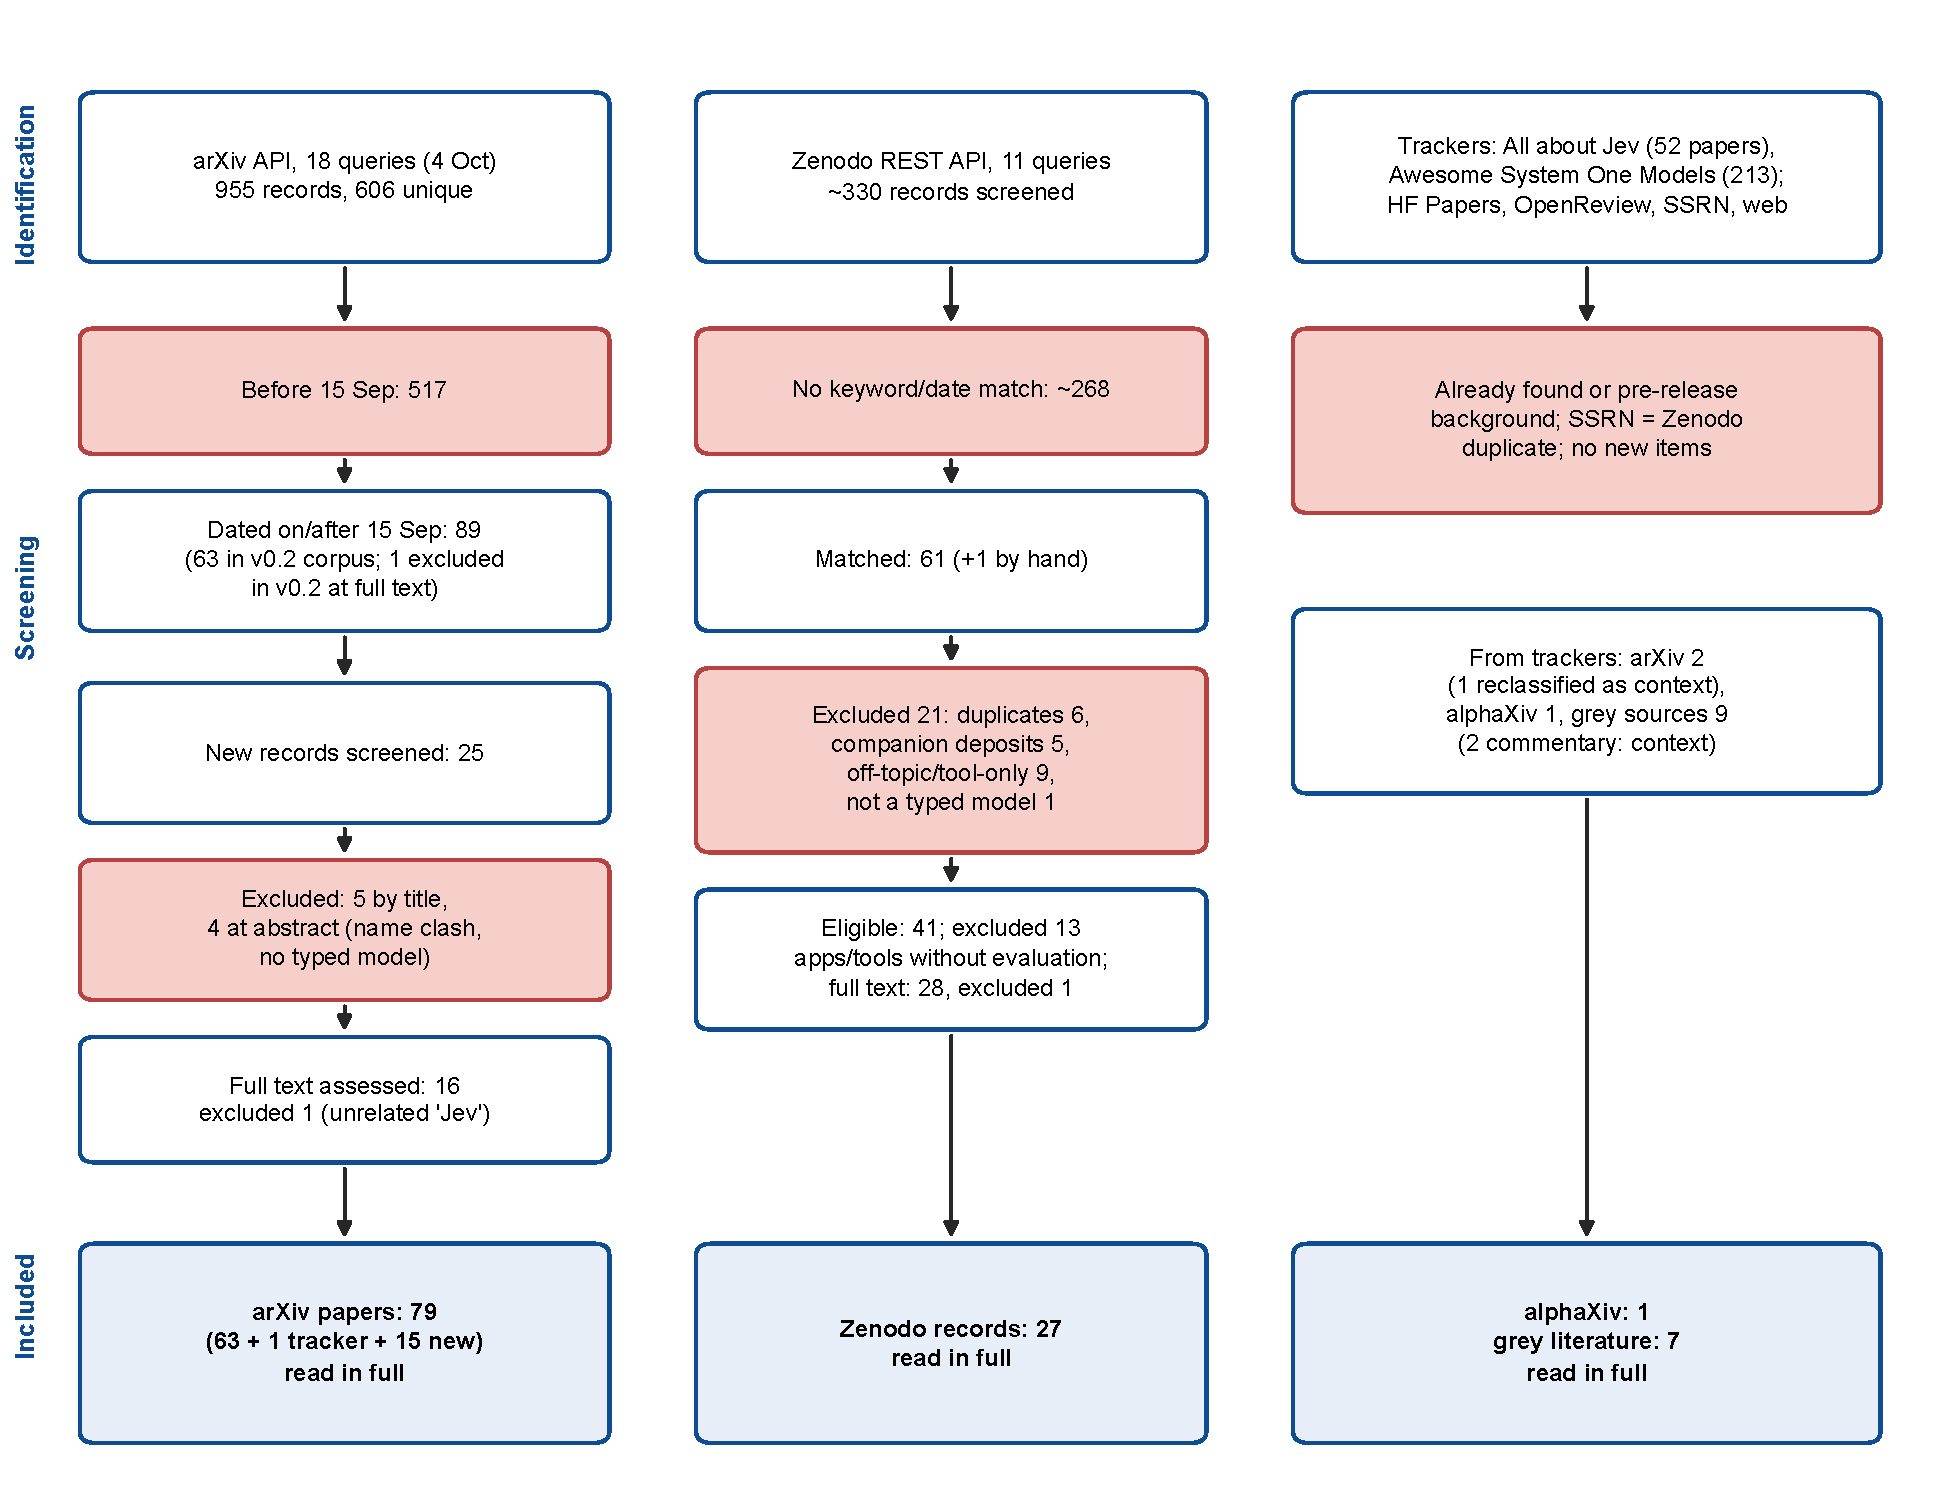
\includegraphics[width=0.85\linewidth]{figures/fig_prisma.pdf}
\caption{Identification, screening and inclusion by source (PRISMA 2020 flow). Zenodo counts at the first step are approximate because the API returns overlapping result sets.}
\label{fig:prisma}
\end{figure}

\paragraph{PRISMA 2020 checklist.}
\Cref{tab:prisma} maps the PRISMA~2020 items~\cite{page2021prisma} to this paper; items that were not done are stated as such.

\begingroup
\small
\renewcommand{\arraystretch}{1.15}
\begin{longtable}{@{}p{0.30\linewidth}p{0.64\linewidth}@{}}
\caption{PRISMA 2020 items and where they are reported.}\label{tab:prisma}\\
\toprule
Item & Where reported, or status \\
\midrule
\endfirsthead
\toprule
Item & Where reported, or status \\
\midrule
\endhead
\bottomrule
\endfoot
Title (1) & Not followed by design: the paper is a policy analysis, and its evidence component is identified as a structured rapid evidence assessment in \cref{sec:method} \\
Abstract (2) & Abstract states question, sources, method, main results, certainty and implications \\
Rationale, objectives (3--4) & \Cref{sec:intro} (research question) \\
Eligibility criteria (5) & \Cref{sec:method}, Eligibility \\
Information sources, search (6--7) & \Cref{sec:method}; \cref{app:queries}; \nolinkurl{scripts/rerun_arxiv_search.py} \\
Selection process (8) & \Cref{sec:method} (Reviewers and tools): AI agents; no duplicate human screening \\
Data collection, items (9--10a/b) & \Cref{sec:method}, Data extraction; \nolinkurl{data/evidence_coding.csv} \\
Study risk of bias (11) & Design appraisal (\cref{sec:appraisal}); \nolinkurl{data/quality_appraisal.csv} \\
Effect measures (12) & Not applicable: direction of the primary result per requirement; no pooled effect \\
Synthesis: eligibility for each synthesis (13a) & Studies coded for a requirement (\cref{app:evidence}) \\
Synthesis: data preparation (13b) & Codes and comparator fields from the extraction; no conversion \\
Synthesis: tabulation and display (13c) & \Cref{fig:framework}, \cref{tab:keyfindings} and \cref{tab:evidence} \\
Synthesis: methods (13d) & Vote counting of direction following SWiM~\cite{campbell2020swim}; no meta-analysis \\
Synthesis: heterogeneity (13e) & Not done formally; heterogeneity of tasks and models is described in \cref{sec:evidence} \\
Synthesis: sensitivity analyses (13f) & Stronger-design studies only; Zenodo records excluded (\cref{sec:across}) \\
Reporting bias (14) & Not formally assessed; discussed in \cref{sec:discussion} \\
Certainty assessment (15) & GRADE-style rules (\cref{sec:appraisal}); \cref{tab:keyfindings} \\
Study selection (16a) & \Cref{fig:prisma} \\
Excluded studies that appear eligible (16b) & \nolinkurl{data/excluded_records.csv} (e.g.\ the unrelated ``Jev'' paper, the mismatched PDF and the harness paper without a typed model) \\
Study characteristics (17) & \Cref{app:evidence,app:catalogue} \\
Risk of bias in studies (18) & \Cref{tab:evidence}; \nolinkurl{data/quality_appraisal.csv} \\
Results of individual studies (19) & \Cref{sec:evidence}; rationales in \nolinkurl{data/evidence_coding.csv} \\
Results of syntheses (20a--d) & \Cref{sec:evidence,sec:across}; \cref{fig:framework}; heterogeneity and formal tests not done \\
Reporting biases (21) & Not assessed formally (\cref{sec:discussion}) \\
Certainty of evidence (22) & \Cref{tab:keyfindings} \\
Discussion (23a--d) & \Cref{sec:discussion} (interpretation, limitations of evidence and of the process, implications) \\
Registration and protocol (24a--c) & Not registered; no protocol published; changes from the earlier release in \cref{sec:method} \\
Support (25) & No funding \\
Competing interests (26) & Positionality and competing interests statement \\
Availability of data, code and materials (27) & Data and code availability statement \\
\end{longtable}
\endgroup
